%!TEX program = xelatex
\documentclass[lang=cn]{elegantpaper}

\title{ElegantPaper: 一个优美的 \LaTeX{} 工作论文模板}
\author{\href{https://ddswhu.me/}{邓 东 升}\thanks{感谢 Peiyi Yao 的帮助与建议。}}

\institute{\href{https://elegantlatex.org/}{Elegant\LaTeX{} 项目组}}
\version{0.05x}
\date{\today}


\begin{document}

\maketitle

\begin{abstract}
\noindent 本文为 \href{https://github.com/ElegantLaTeX/ElegantPaper/}{ElegantPaper} 的说明文档(中文)。此模板基于 \LaTeX{} 的 article 类,专为工作论文写作而设计。设计这个模板的初衷是让作者不用关心工作论文的格式,专心写作,从而有更加舒适,简便的写作体验。如果你有其他问题、建议或者报告 bug,可以在 \href{https://github.com/ElegantLaTeX/ElegantPaper/issues}{ElegantPaper/issues} 留言。如果你想了解更多由 Elegant\LaTeX{} 项目组设计的模板,请访问 \href{https://github.com/ElegantLaTeX/}{https://github.com/ElegantLaTeX/}。
\keywords{Elegant\LaTeX{},工作论文,模板}
\end{abstract}

\section{模板介绍}

此模板是基于 \LaTeX{} 的标准文档类设计,也即意味着你可以在在文类选项使用文档(article)类型的选项,比如 \lstinline{a4paper, 12pt} 等等。本模板支持 \lstinline{PDFLaTeX} 和 \lstinline{XeLaTeX} 两种编译方式。
      
\subsection{全局选项}
我在这个模板中定义了一个语言选项 \lstinline{lang},可以选择英文模式 \lstinline{lang=en}(默认)或者中文模式 \lstinline{lang=cn}。当选择中文模式时,图表的标题引导词以及参考文献,定理引导词等信息会变成中文。你可以通过下面两种方式来选择语言模式:
\begin{lstlisting}
\documentclass[lang=cn]{elegantpaper}
\documentclass{cn}{elegantpaper} % 两者皆可
\end{lstlisting}

\subsection{字体设置}
\subsubsection[选择 PDFLaTeX 编译]{选择 \lstinline{PDFLaTeX} 编译}
如果你使用 \lstinline{PDFLaTeX} 编译,默认的 Computer Modern 字体被换成了 \lstinline{newtx} 系列字体,默认的字体字号是 11 pt。关于字体设置的宏包主要用到了:
\begin{itemize}
	\item \lstinline{newtxtext} 用于文档正文字体,类似于 Times New Roman 字体。
	\item \lstinline{newtxmath} 用于数学字体,搭配 \lstinline{newtx} 非常合适,类似于过时的 \lstinline{times} 宏包的效果。
	\item \lstinline{FiraMono} 用于打字机字体,并使用了 \lstinline{scale=0.8} 选项。
	\item \lstinline{ctex} 用于中文字体设置,并使用了 \lstinline{scheme=plain} 选项。
\end{itemize}

\subsubsection[选择 XeLaTeX 编译]{选择 \lstinline{XeLaTeX} 编译}
如果你选择 \lstinline{XeLaTeX} 编译的话,那么设置字体的宏包为 \lstinline{fontspec} 和 \lstinline{xeCJK}。由于模板中使用的字体是 Windows 中的字体,所以如果你使用其他操作系统,比如 Linux 或者 Mac OS,那么你需要把所用字体替换为你系统中的字体。设置字体的命令:

\begin{lstlisting}
\RequirePackage{fontenc}
\RequirePackage[no-math]{fontspec}
\setmainfont{Times New Roman}[NFSSFamily=ntxtlf]
\setsansfont{Arial}
%\setmonofont[Scale=0.9]{Courier New}
\RequirePackage{xeCJK}
\RequirePackage{xunicode}
\setCJKmainfont[BoldFont={SimHei},ItalicFont={KaiTi}]{SimSun}
\setCJKsansfont[BoldFont={SimHei},ItalicFont={KaiTi}]{KaiTi}
\setCJKmonofont[BoldFont={SimHei},ItalicFont={KaiTi},Scale=0.9]{Microsoft YaHei}
\XeTeXlinebreaklocale "zh"
\XeTeXlinebreakskip = 0pt plus 1pt minus 0.1pt
\RequirePackage{newtxmath}
\end{lstlisting}

\subsubsection{其他设置}

这几个包由于都是一个系列的,字体搭配起来非常合适,字体宽度非常契合!唯独数学字体中的大型运算符,比如求和符号和积分符号不是很好看,为此,我把它们又改回了原先的字体效果。公式~(\ref{eq:binom}) 展示了最终的数学字体的效果。
\begin{equation}
(a+3b)^{n} = \sum_{k=0}^{n} C_{n}^{k} a^{n-k} (3b)^k \label{eq:binom}
\end{equation}

我把行距设定为 1.3,并且使用了 \lstinline{microtype} 宏包调整字体的间距,为了去除字体字号,字形警告信息,我使用了 \lstinline{type1cm} 宏包。


\subsection{自定义命令}
在此模板中,并没有修改任何默认的命令或者环境,所以,你可以在此模板使用原来的命令和环境。另外,我自定义了 3 个命令:

\begin{enumerate}
	\item \lstinline{\email}:创建邮箱地址的链接;
	\item \lstinline{\figref}:用法和 \lstinline{\ref} 类似,但是会在插图的标题前添加 <\textbf{图 n}> ;
	\item \lstinline{\tabref}:用法和 \lstinline{\ref} 类似,但是会在表格的标题前添加 <\textbf{表 n}>;
	\item \lstinline{\keywords}:为摘要环境添加关键词。
\end{enumerate}



\subsection{列表环境}
你可以使用列表环境(\lstinline{itemize}、\lstinline{enumerate}、\lstinline{description}),示例如下:\\[2ex]
\begin{minipage}[c]{0.51\linewidth}
\begin{lstlisting}
\begin{itemize}
	\item 春花秋月何时了, 往事知多少? 
	\item 小楼昨夜又东风, 故国不堪回首月明中。
	\item 雕栏玉砌应犹在, 只是朱颜改。
	\item 问君能有几多愁?恰似一江春水向东流。
\end{itemize}
\end{lstlisting}
\end{minipage}
\begin{minipage}[c]{0.48\linewidth}
\begin{itemize}
	\item 春花秋月何时了, 往事知多少? 
	\item 小楼昨夜又东风, 故国不堪回首月明中。
	\item 雕栏玉砌应犹在, 只是朱颜改。
	\item 问君能有几多愁?恰似一江春水向东流。
\end{itemize}
\end{minipage}




\subsection{插图}
插图的命令和以前一样,也是使用 \lstinline{figure} 环境。\figref{fig:scatter} 显示了插图的效果。你可以把你的图放到当前工作目录的如下子目录下 (\lstinline{./image/}, \lstinline{./img/}, \lstinline{./figure/}, \lstinline{./fig/})。

\begin{lstlisting}
% 如果要使抄录环境显示中文,必须用 XeLaTeX,而不能用 PDFLaTeX
% 这是由于 lstlisting 和 ctex 的问题
\begin{figure}[htbp]
	\centering
	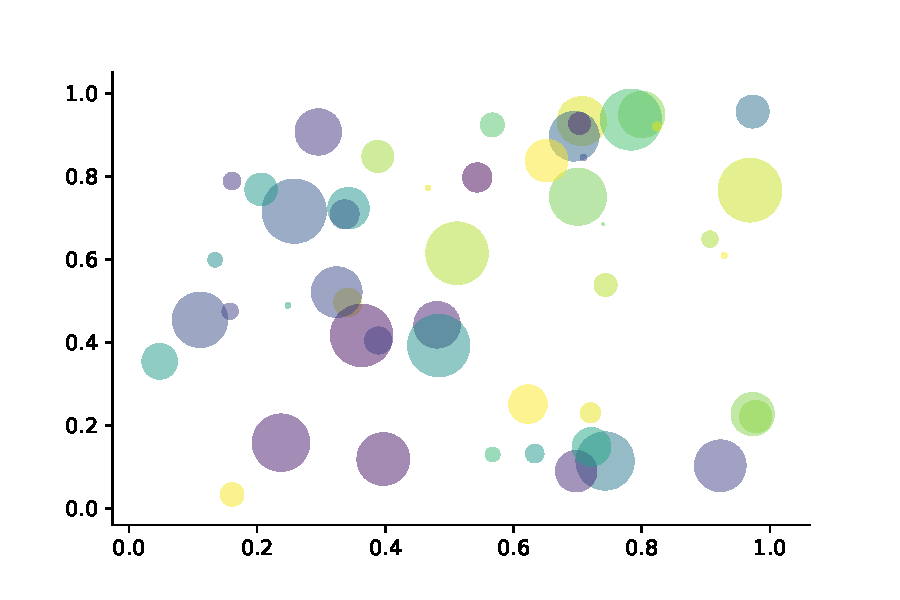
\includegraphics[width=0.6\textwidth]{scatter.pdf}
	\caption{散点图示例\label{fig:scatter}} 
\end{figure}
\end{lstlisting}

\begin{figure}[htbp]
	\centering
	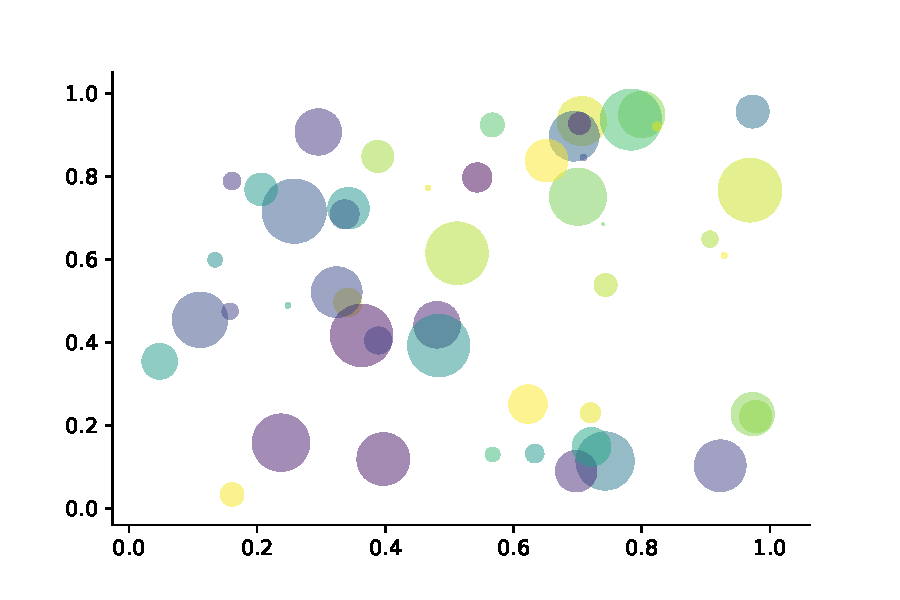
\includegraphics[width=0.6\textwidth]{scatter.pdf}
	\caption{散点图示例\label{fig:scatter}}
\end{figure}


\subsection{表格}
我强烈建议你使用 \lstinline{booktabs} 宏包,这个宏包有三个命令 \lstinline{\toprule}、\lstinline{\midrule} 和 \lstinline{\bottomrule} 能方便你制作三线表。\tabref{tab:reg} 是一个示例:

\begin{lstlisting}
\begin{table}[htbp]
  \small
  \centering
  \caption{燃油效率与汽车价格}
    \begin{tabular}{lcc}
    \toprule
                    &       (1)         &        (2)      \\
    \midrule
    燃油效率        &    -238.90***     &      -49.51     \\
                    &     (53.08)       &      (86.16)    \\
    汽车重量        &                   &        1.75***  \\
                    &                   &       (0.641)   \\
    常数项          &  11,253***        &    1,946       \\
                    &  (1,171)          &   (3,597)      \\
    观测数          &      74           &       74       \\
    $R^2$           &       0.220       &        0.293   \\
    \bottomrule
    \multicolumn{3}{l}{\scriptsize 括号内为标准误} \\
    \multicolumn{3}{l}{\scriptsize *** p<0.01, ** p<0.05, * p<0.1} \\
    \end{tabular}%
  \label{tab:reg}%
\end{table}%
\end{lstlisting}

\begin{table}[htbp]
  \small
  \centering
  \caption{燃油效率与汽车价格}
    \begin{tabular}{lcc}
    \toprule
                    &       (1)         &        (2)      \\
    \midrule
    燃油效率        &    -238.90***     &      -49.51     \\
                    &     (53.08)       &      (86.16)    \\
    汽车重量        &                   &        1.75***  \\
                    &                   &       (0.641)   \\
    常数项          &  11,253***        &    1,946       \\
                    &  (1,171)          &   (3,597)      \\
    观测数          &      74           &       74        \\
    $R^2$           &       0.220       &        0.293    \\
    \bottomrule
    \multicolumn{3}{l}{\scriptsize 括号内为标准误} \\
    \multicolumn{3}{l}{\scriptsize *** p<0.01, ** p<0.05, * p<0.1} \\
    \end{tabular}%
  \label{tab:reg}%
\end{table}%


\subsection{参考文献}
此模板使用了 Bib\TeX{} 来生成参考文献,默认使用的文献样式(bib style)是 \lstinline{aer}。参考文献示例:~\cite{Chen2018} 使用了中国一个大型的 P2P 平台(人人贷)的数据来检验男性投资者和女性投资者在投资表现上是否有显著差异。

你可以在谷歌学术,Mendeley,Endnote 中获得文献条目(bib item),然后把它们添加到 \lstinline{wpref.bib} 中。在文中引用的时候,引用它们的键值(bib key)即可。注意需要在编译的过程中添加 Bib\TeX{} 编译。如果你想在参考文献中添加未引用的文献,可以使用

\begin{lstlisting}
\nocite{EINAV2010, Havrylchyk2018} 
\end{lstlisting}

\section{示例}
在这部分,我提供一个示例文档:

\begin{lstlisting}
\documentclass[lang=cn]{elegantpaper}

% 标题信息
\title{工作论文示例展示}
\author{ddswhu} 
\institute{Elegant\LaTeX{} 项目组}
\version{1.00}
\date{\today}

\begin{document}

\maketitle

\begin{abstract}
在这里写摘要。
\keywords{关键词1,关键词2}
\end{abstract}

\section{引言}
这一部分是引言的内容。

\section{结论}
这是结论部分。

% 在参考文献部分显示未引用的文献
\nocite{ref1, ref2}
% 生成参考文献
\bibliography{wpref}
\end{document}
\end{lstlisting}

\nocite{EINAV2010,Havrylchyk2018} 
\bibliography{wpref}

\end{document}
